\documentclass{article}
\usepackage[a4paper, margin=2.5cm]{geometry}
\usepackage{graphicx}
\usepackage{pgf}
\usepackage{pgfkeys}
\usepackage{caption}
\usepackage{amsfonts}
\usepackage{xcolor}
\usepackage{amsmath}
\usepackage{amsthm}
\usepackage{hyperref}
\usepackage{cleveref}
\usepackage{enumitem}
\usepackage{float}
\usepackage{diagbox}
\usepackage{tikz}
\usepackage{adjustbox}
\usepackage{pgfplots}
\usepackage{placeins} % To use \FloatBarrier
\usetikzlibrary{arrows.meta, positioning}

\hypersetup{
    colorlinks=true,
    linkcolor=blue,
    filecolor=magenta,
    urlcolor=cyan,
    citecolor=blue
}

\newtheorem{theorem}{Theorem}[section]  % Theorems numbered within sections
\newtheorem{lemma}[theorem]{Lemma}      % Lemma numbering follows theorem

% Define argmax
\DeclareMathOperator*{\argmax}{arg\,max}  % The asterisk is used to allow limits to go underneath in displaystyle

% Apply color to cref and Cref
\crefformat{figure}{#2figure\color{blue}~#1#3}
\Crefformat{figure}{#2Figure\color{blue}~#1#3}
\crefformat{section}{#2section\color{blue}~#1#3}
\Crefformat{section}{#2Section\color{blue}~#1#3}
\crefformat{table}{#2table\color{blue}~#1#3}
\Crefformat{table}{#2Table\color{blue}~#1#3}

% color definitions
\definecolor{darkgreen}{rgb}{0.0, 0.7, 0.0} % A darker green

% Define the keys used in the graph
\pgfkeys{
    /graph/.is family, /graph,
    default/.style={
        buyers={}, 
        items={}, 
        buyerValues={}, 
        prices={},
        priceVectorName=p % Default name
    },
    buyers/.estore in=\GraphBuyers,
    items/.estore in=\GraphItems,
    buyerValues/.estore in=\GraphBuyerValues,
    prices/.estore in=\GraphPrices,
    priceVectorName/.estore in=\GraphPriceVectorName % Store the custom price vector name
}

% Helper macro to extract prices by index
\newcommand{\getPrice}[1]{
    \foreach \price [count=\i] in \GraphPrices {
        \ifnum\i=#1
            \xdef\selectedPrice{\price}
            \breakforeach % Stop the loop once the correct item is found
        \fi
    }
}

% Helper macro to extract values by index
\newcommand{\getValue}[2]{
    \foreach \value [count=\i] in \GraphBuyerValues{
        \ifnum\i=#1
            \foreach \val [count=\j] in \value {
                \ifnum\j=#2
                    \xdef\selectedValue{\val}
                    \breakforeach % Stop the loop once the correct item is found
                \fi
            }
        \fi
    }
}

% Helper macro to extract utilities by index
\newcommand{\getUtility}[2]{
    \getPrice{#2}  % Retrieve the price by index
    \getValue{#1}{#2}  % Retrieve the values by index
    \pgfmathsetmacro\utility{int(\selectedValue - \selectedPrice)} % Ensure result is an integer
}

% Helper macro to extract the indices of the maximum non-negative utilities for a buyer
\newcommand{\getPreferredUtilityIndices}[1]{
    \global\def\maxUtility{0} % Initialize maxUtility globally
    \def\preferredItems{-1} % List to store all best items
    \foreach \item [count=\ii] in \GraphItems {
        \typeout{currindices={\bi, \ii}}
        % Compute utility
        \getUtility{#1}{\ii} % Retrieve the utility by indices
        \typeout{utility={\utility}}

        % Check if this utility is the maximum for this buyer
        \ifnum\utility>\maxUtility
            \xdef\maxUtility{\utility}
            \xdef\preferredItems{\ii} % Reset with the new best item
        \else
            \ifnum\utility=\maxUtility
                \xdef\preferredItems{\preferredItems, \ii} % Append this item to the list
            \fi
        \fi
    }
    \typeout{Max Utility for \buyer: \maxUtility, Best Items: \preferredItems}
}

% Helper macro to extract the indices of non-negative utilities for a buyer
\newcommand{\getAcceptableUtilityIndices}[1]{
    \def\acceptableItems{-1} % List to store all acceptable items
    \foreach \item [count=\ii] in \GraphItems {
        \typeout{currindices={\bi, \ii}}
        % Compute utility
        \getUtility{#1}{\ii} % Retrieve the utility by indices
        \typeout{utility={\utility}}

        % Check if this utility is non-negative
        \ifnum\utility<0
        \else
            \xdef\acceptableItems{\acceptableItems, \ii} % Append this item to the list
        \fi
    }
    \typeout{Acceptable Items for \buyer: \acceptableItems}
}

% New macro to construct "\item : \value" list
\newcommand{\getValueDict}[1]{
    \def\valueList{}% Global definition to ensure it is accessible outside the scope of this macro
    \foreach \item [count=\ii] in \GraphItems {
        \getValue{#1}{\ii}% This should set \selectedValue appropriately
        \typeout{value={\selectedValue}}
        \ifnum\ii=1
            \xdef\valueList{\item: \selectedValue}
        \else
            \xdef\valueList{\valueList, \item: \selectedValue}
        \fi
    }
}

% New macro to construct "\item : \utility" acceptability list
\newcommand{\getAcceptableUtilityDict}[1]{
    \def\utilityList{}% Global definition to ensure it is accessible outside the scope of this macro
    \foreach \item [count=\ii] in \GraphItems {
        \getUtility{#1}{\ii}% This should set \utility appropriately
        \xdef\utilityString{\item: \utility} % Use \edef for expanded definition
        \ifnum\utility < 0
        \else
            \xdef\utilityString{\item: \textcolor{darkgreen}{\utility}} % Color non-negative utilities
        \fi
        \ifnum\ii=1
            \xdef\utilityList{\utilityString} % Initialize utilityList with the first item
        \else
            \xdef\utilityList{\utilityList, \utilityString} % Append subsequent items
        \fi
    }
}

% New macro to get max non-negative utility
\newcommand{\getMaxUtility}[1]{
    \def\maxUtility{-1} % Initialize maxUtility
    \foreach \item [count=\ii] in \GraphItems {
        \getUtility{#1}{\ii} % Retrieve the utility by index
        \ifnum\utility<0
        \else
            \ifnum\utility>\maxUtility
                \xdef\maxUtility{\utility}
            \fi
        \fi
    }
}

% New macro to construct "\item : \utility" preferred list
\newcommand{\getPreferredUtilityDict}[1]{
    \def\utilityList{}% Global definition to ensure it is accessible outside the scope of this macro
    \getMaxUtility{#1} % Retrieve the maximum non-negative utility
    \foreach \item [count=\ii] in \GraphItems {
        \getUtility{#1}{\ii}% This should set \utility appropriately
        \xdef\utilityString{\item: \utility} % Use \edef for expanded definition
        \ifnum\utility < 0 % only non-negative utilities can be preferred
        \else
            \ifnum\utility = \maxUtility

                \xdef\utilityString{\item: \textcolor{darkgreen}{\utility}} % Color non-negative utilities
            \fi
        \fi
        \ifnum\ii=1
            \xdef\utilityList{\utilityString} % Initialize utilityList with the first item
        \else
            \xdef\utilityList{\utilityList, \utilityString} % Append subsequent items
        \fi
    }
}

% Define the command to create the graph
\newcommand{\createPreferredGraph}[1]{
    \pgfkeys{/graph/.cd,#1}  % Apply settings within the /graph family
    \expandafter\parsePreferredGraphData\expandafter{\GraphBuyers}{\GraphItems}{\GraphBuyerValues}{\GraphPrices}{\GraphPriceVectorName}
}

% Helper macro to process the graph data and render the tikzpicture
\newcommand{\parsePreferredGraphData}[5]{
    \begin{figure}[H]
        \centering
        \begin{tikzpicture}[every node/.style={align=center}]
            % Define nodes for buyers
            \typeout{msg={#1}}
            \foreach \buyer [count=\bi] in {#1} {
                \node[draw, circle] (buyer-\bi) at (0, {-2*\bi}) {\buyer};
            }
            % Define nodes for items
            \typeout{msg={#2}}
            \typeout{msg={#4}}
            \foreach \item [count=\ii] in #2 {
                \typeout{msg={\ii}}
                \getPrice{\ii}  % Retrieve the price by index
                \node[draw, circle] (item-\ii) at (4, {-2*\ii}) {\item \\ $#5_{\item} = \selectedPrice$};
            }
            % Calculate utilities and draw preferred choices
            \foreach \buyer [count=\bi] in {#1} {

                % Get indices of preferred items
                \getPreferredUtilityIndices{\bi}

                % Draw edges to preferred items
                \typeout{preferred={Preferred Items: \preferredItems}}
                \foreach \ii in \preferredItems {
                    \ifnum\ii > 0
                        \draw (buyer-\bi) -- (item-\ii);
                    \fi
                }

                % List values and utilities
                \getValueDict{\bi}
                \getPreferredUtilityDict{\bi}

                \node[anchor=east] at (-1, {-2*\bi + 0.3}) {Values for $\buyer$: $\{\valueList\}$};
                \node[anchor=east] at (-1, {-2*\bi - 0.3}) {Utility for $\buyer$: $\{\utilityList\}$};
            }
        \end{tikzpicture}
    \end{figure}
}

% Define the command to create the graph
\newcommand{\createAcceptabilityGraph}[1]{
    \pgfkeys{/graph/.cd,#1}  % Apply settings within the /graph family
    \expandafter\parseAcceptabilityGraphData\expandafter{\GraphBuyers}{\GraphItems}{\GraphBuyerValues}{\GraphPrices}{\GraphPriceVectorName}
}

% Helper macro to process the graph data and render the tikzpicture
\newcommand{\parseAcceptabilityGraphData}[5]{
    \begin{figure}[H]
        \centering
        \begin{tikzpicture}[every node/.style={align=center}]
            % Define nodes for buyers
            \typeout{msg={#1}}
            \foreach \buyer [count=\bi] in {#1} {
                \node[draw, circle] (buyer-\bi) at (0, {-2*\bi}) {\buyer};
            }
            % Define nodes for items
            \typeout{msg={#2}}
            \typeout{msg={#4}}
            \foreach \item [count=\ii] in #2 {
                \typeout{msg={\ii}}
                \getPrice{\ii}  % Retrieve the price by index
                \node[draw, circle] (item-\ii) at (4, {-2*\ii}) {\item \\ $#5_{\item} = \selectedPrice$};
            }
            % Calculate utilities and draw acceptable choices
            \foreach \buyer [count=\bi] in {#1} {

                % Get indices of acceptable items
                \getAcceptableUtilityIndices{\bi}

                % Draw edges to acceptable items
                \typeout{acceptable={Acceptable Items: \acceptableItems}}
                \foreach \ii in \acceptableItems {
                    \ifnum\ii > 0
                        \draw (buyer-\bi) -- (item-\ii);
                    \fi
                }

                % List values and utilities
                \getValueDict{\bi}
                \getAcceptableUtilityDict{\bi}

                \node[anchor=east] at (-1, {-2*\bi + 0.3}) {Values for $\buyer$: $\{\valueList\}$};
                \node[anchor=east] at (-1, {-2*\bi - 0.3}) {Utility for $\buyer$: $\{\utilityList\}$};
            }
        \end{tikzpicture}
    \end{figure}
}

% start
\title{
    Homework Assignment 3 - Coding Part Write-up\\
    Networks and Markets
}
\author{
    Omer Zohar
    \and
    Gil Aharoni
    \and
    Adam Tuby
}

\bibliographystyle{plain}

\begin{document}
\maketitle

\section*{Part 4: Implementing Matching Market Pricing}
\setcounter{section}{0}


\section{Question 7}

\begin{enumerate}[label=(\alph*)]

    \item[(b)] Consider the matching market example in Lecture 5 Page 7:
    
    \begin{figure}[h]
        \centering
        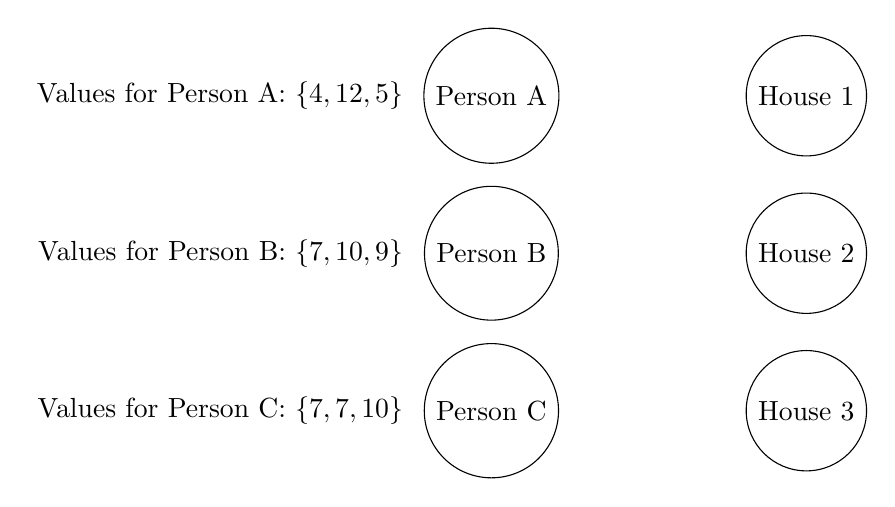
\begin{tikzpicture}
            % Define nodes for buyers
            \node[draw, circle] (buyer-1) at (0, 0) {Person A};
            \node[draw, circle] (buyer-2) at (0, -2) {Person B};
            \node[draw, circle] (buyer-3) at (0, -4) {Person C};
            % Define nodes for items
            \node[draw, circle, align=center] (item-1) at (4, 0) {House 1};
            \node[draw, circle, align=center] (item-2) at (4, -2) {House 2};
            \node[draw, circle, align=center] (item-3) at (4, -4) {House 3};
            % Output values
            \node[anchor=east] at (-1, 0) {Values for Person A: $\{4, 12, 5\}$};
            \node[anchor=east] at (-1, -2) {Values for Person B: $\{7, 10, 9\}$};
            \node[anchor=east] at (-1, -4) {Values for Person C: $\{7, 7, 10\}$};
        \end{tikzpicture}
    \end{figure}

    Formally, the matching market context is $\Gamma = (\{A, B, C\}, \{1, 2, 3\}, v)$, where $v$ is the valuation function defined as follows:

    \begin{align*}
        v_A(1) &= 4, v_A(2) = 12, v_A(3) = 5 \\
        v_B(1) &= 7, v_B(2) = 10, v_B(3) = 9 \\
        v_C(1) &= 7, v_C(2) = 7, v_C(3) = 10
    \end{align*}

    We turn to run the algorithm of Theorem 8.8 to find a market equilibrium $(p, M)$ to find the maximum social value, in order to validate out implementation's output. We begin by initializing the prices vector $\vec{p} \equiv 0$ to be the zero vector. We then proceed to run the algorithm, updating the prices vector until there is a perfect matching $M$ in the induced preferred choice graph for $(\Gamma, \vec{p})$:

    \begin{enumerate}[label=\arabic*.]

        \item Observing the following \textit{induced preferred-choice graph} from $(\Gamma, \vec{p})$:
        
        \createPreferredGraph{
            buyers={A, B, C},
            items={1, 2, 3},
            buyerValues={{4, 12, 5}, {7, 10, 9}, {7, 7, 10}},
            prices={0, 0, 0},
            priceVectorName=p
        }

        There obviously isn't a perfect matching as $S = \{A, B\}$ is a constricted set with $\left|N(S)\right| = \left|\{2\}\right| = 1 < 2 = \left|S\right|$ (which, by a theorem we've seen in class, implies that there isn't a perfect matching). Thus, we raise the prices for all items in $N(S)$ by 1, and update the prices vector $\vec{p}$ accordingly. The updated prices vector is $\vec{p} = (a: 0, b: 1, c: 0)$. Not all prices are greater than zero, so we don't perform a shift operation, and we proceed to the next iteration.

        \item Observing the following \textit{induced preferred-choice graph} from $(\Gamma, \vec{p})$:
        
        \createPreferredGraph{
            buyers={A, B, C},
            items={1, 2, 3},
            buyerValues={{4, 12, 5}, {7, 10, 9}, {7, 7, 10}},
            prices={0, 1, 0},
            priceVectorName=p
        }

        There obviously isn't a perfect matching as $S = \{A, B, C\}$ is a constricted set with $\left|N(S)\right| = \left|\{2, 3\}\right| = 2 < 3 = \left|S\right|$ (which, by a theorem we've seen in class, implies that there isn't a perfect matching). Thus, we raise the prices for all items in $N(S)$ by 1, and update the prices vector $\vec{p}$ accordingly. The updated prices vector is $\vec{p} = (a: 0, b: 2, c: 1)$. Not all prices are greater than zero, so we don't perform a shift operation, and we proceed to the next iteration.

        \item Observing the following \textit{induced preferred-choice graph} from $(\Gamma, \vec{p})$:
        
        \createPreferredGraph{
            buyers={A, B, C},
            items={1, 2, 3},
            buyerValues={{4, 12, 5}, {7, 10, 9}, {7, 7, 10}},
            prices={0, 2, 1},
            priceVectorName=p
        }

        Similar to the previous iteration, we raise the prices for $\{2, 3\}$, and update the prices vector $\vec{p}$ accordingly. The updated prices vector is $\vec{p} = (a: 0, b: 3, c: 2)$. Not all prices are greater than zero, so we don't perform a shift operation, and we proceed to the next iteration.

        \item Observing the following \textit{induced preferred-choice graph} from $(\Gamma, \vec{p})$:
        
        \createPreferredGraph{
            buyers={A, B, C},
            items={1, 2, 3},
            buyerValues={{4, 12, 5}, {7, 10, 9}, {7, 7, 10}},
            prices={0, 3, 2},
            priceVectorName=p
        }

        And there is a perfect matching in the induced preferred choice graph, which is $M = \{\{A, 2\}, \{B, 1\}, \{C, 3\}\}$. Thus, the market equilibrium is $(\vec{p}, M) = ((1: 0, 2: 3, 3: 2), \{\{A, 2\}, \{B, 1\}, \{C, 3\}\})$, and we are done.
    \end{enumerate}

    We found the market equilibrium to be $(\vec{p}, M) = ((1: 0, 2: 3, 3: 2), \{\{A, 2\}, \{B, 1\}, \{C, 3\}\})$. The maximum social value is therefore $v(A, 2) + v(B, 1) + v(C, 3) = 12 + 7 + 10 = 29$.

    Our algorithm found exactly this market equilibrium.

\end{enumerate}

\section{Question 8}

\begin{enumerate}[label=(\alph*)]

    \item 

    
    \item 


\end{enumerate}

\section{Bonus Question 2}

\begin{enumerate}[label=(\alph*)]

    \item 

    
    \item 


    \item 

    
    \item 


\end{enumerate}

\section*{Part 5: Exchange Networks for Uber}
\setcounter{section}{0}


\section{Question 9}

\section{Question 10}

\begin{enumerate}[label=(\alph*)]

    \item 

    
    \item 


\end{enumerate}


\section{Question 11}

\section{Bonus Question 3}

\begin{enumerate}[label=(\alph*)]

    \item 

    
    \item 

\end{enumerate}

\bibliography{bibliography}

\end{document}